\begin{figure}[H]
  \centering
  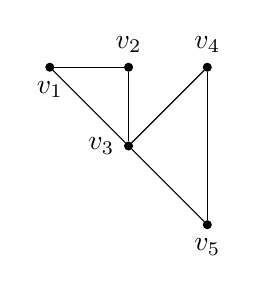
\begin{tikzpicture}
  \tikzset{enclosed/.style={draw, circle, inner sep=0pt, minimum size=.10cm, fill=black}}
  	\node[enclosed] at (0,2) (v_1) [label=below:\(v_1\)] {};
    \node[enclosed] at (1,2) (v_2) [label=above:\(v_2\)] {};
    \node[enclosed] at (1,1) (v_3) [label=left:\(v_3\)] {};
    \node[enclosed] at (2,2) (v_4) [label=above:\(v_4\)] {};
    \node[enclosed] at (2,0) (v_5) [label=below:\(v_5\)] {};
    
    \footnotesize
    \draw (v_1) -- (v_2);
    \draw (v_1) -- (v_3);
    \draw (v_2) -- (v_3);
    \draw (v_3) -- (v_4);
    \draw (v_3) -- (v_5); 
    \draw (v_4) -- (v_5);
  \end{tikzpicture}